\chapter{Ergebnisse}
\section{Daten und Beobachtungen}
Über die $T = 10000$ Trainingsepisoden wurden folgende durchschnittliche Belohnungen pro Epsiode berechnet:
\begin{table}[H]
    \centering
    \begin{tabular}{c|c}
            & $\frac{\sum r}{T}$ \\
        \hline
        QLearningAgent($\alpha$ = 0.1, $\gamma$ = 0.95)  & 265 \\
        \hline
        DeepQLearningAgent($\alpha$ = 0.001, $\gamma$ = 0.95) & 287 \\
        \hline
        RandomStrategies & 233
    \end{tabular}
    \caption{Trainigs-Ergebnisse}
    \label{table:trainingsergebnisse}
\end{table}
Es bildet sich also schon während des Trainings ab, dass der QLearning-Agent und der Deep QLearning-Agent langfristig
bessere Entscheidungen treffen, als der \textit{RandomStrategies} Agent. Es lohnt sich also weniger jedes Spiel
eine zufällige etablierte Strategie zu wählen.
Nach dem Training wurden alle Agenten und Strategien in einem Tunier getestet:
\begin{figure}[H]
    \centering
    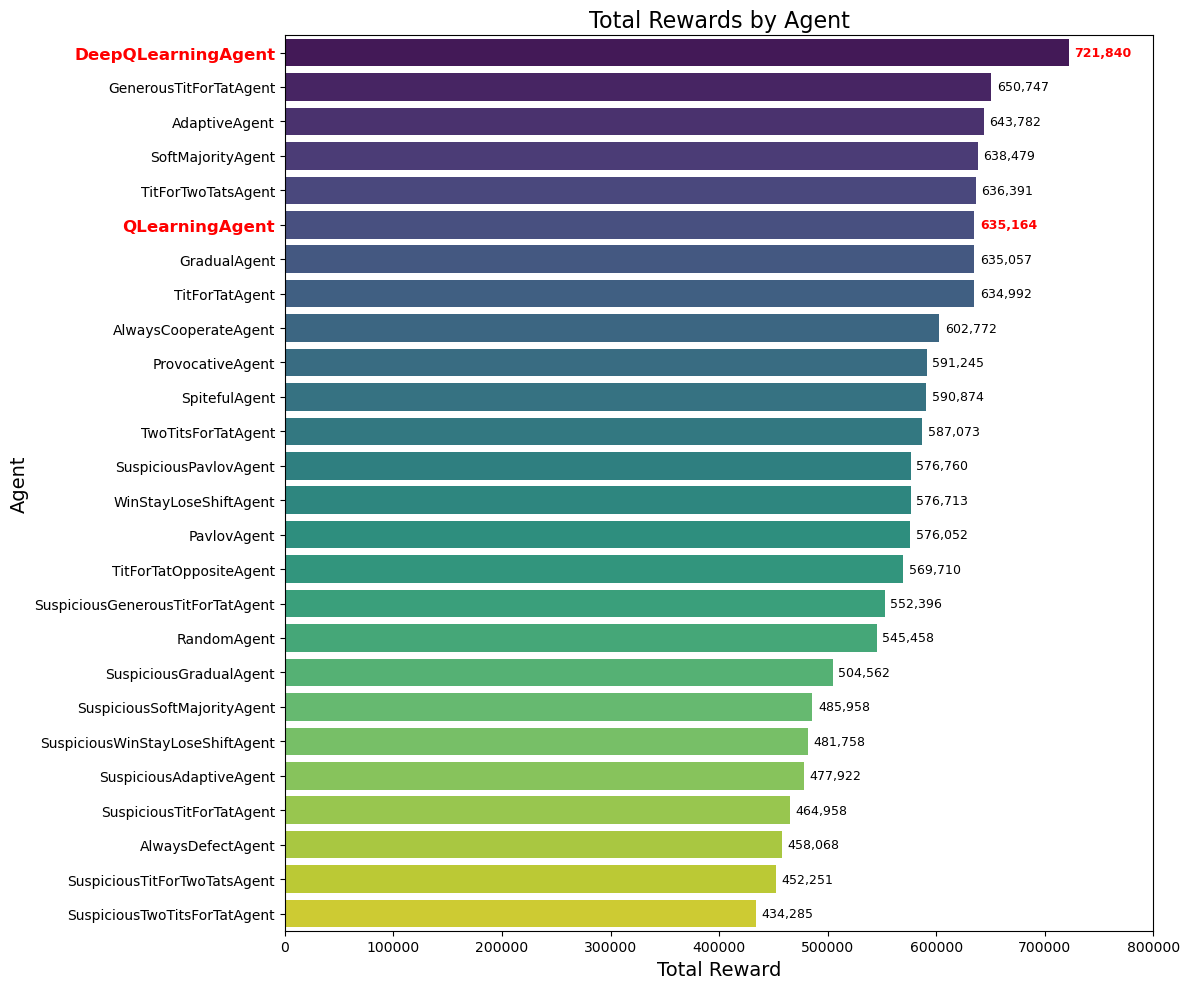
\includegraphics[height=8cm]{../poster/logos/tournament.png}
    \caption{Gesamtbelohnungen der Agenten im Turnier}
    \label{fig:gesamtbelohnungen}
\end{figure}
Bevor die Ergebnisse der RL-Agenten genauer analysiert werden, können einige Beobachtungen zusammengetragen werden:
\begin{itemize}
    \item \textit{Suspicious} Agenten schneiden insgesamt schlechter ab.
    \item Die beste Basis-Strategie ist \textit{GenerousTitForTat}.
    \item Immer zu kooperieren ist besser als immer zu defektieren.
\end{itemize}
Diese Beobachtungen decken sich auch mit den Entdeckungen, die Robert Axelrod in seinem Buch 
\textit{The Evolution of Cooperation}\footcite{axelrod1984cooperation} gemacht hat.

\subsection{QLearning-Ergebnisse}
Aus dem Training ging folgende Q-Tabelle hervor:
\begin{table}[H]
    \centering
    \begin{tabular}{c|c|c}
            & Q-Werte für Kooperation & Q-Werte für Defektion \\
        \hline
        Gegner kooperierte &  52.7929238 & 2.61803697\\
        \hline
        Gegner defektierte &  0.9977664 & 53.59111475 \\
    \end{tabular}
    \caption{Q-Tabelle nach dem Training}
    \label{table:qtableaftertraining}
\end{table}
Da $Q(0, 0) > Q(0, 1) \land Q(1, 0) < Q(1, 1)$ gilt, konvergierte der Q-Learning-Agent offentsichtlich in Richtung des
\textit{TitForTatAgent}'s. Dies spiegelt sich auch in den Tunierergebnissen (siehe Abb. \ref{fig:gesamtbelohnungen}) wieder:
Dort reiht sich der QLearning-Agent auch dort ein. Durch unterschiedliche Entscheidungen von Agenten, die auf Wahrscheinlichkeiten 
beruhen (\textit{RandomAgent, \textit{GenerousTitForTatAgent}}) gibt es minimale Abweichungen zwischen den Agenten.
Wenn man diese Ergebnisse mit denen der anderen drei Strategien, die der \textit{QLearningAgent} entwickeln konnte vergleicht,
fällt auf, dass die TitForTat-Strategie langfristig die besten Ergebnisse erzielt. Es gilt:
\textit{TitForTatAgent} > \textit{AlwaysCooperateAgent} > \textit{TitForTatOppositeAgent} > \textit{AlwaysDefectAgent}.
Die Verteilung von Kooperation und Defektion des Q-Learning-Agenten ist in Abb. \ref{fig:qverteilung} dargestellt:
\begin{figure}[H]
    \centering
    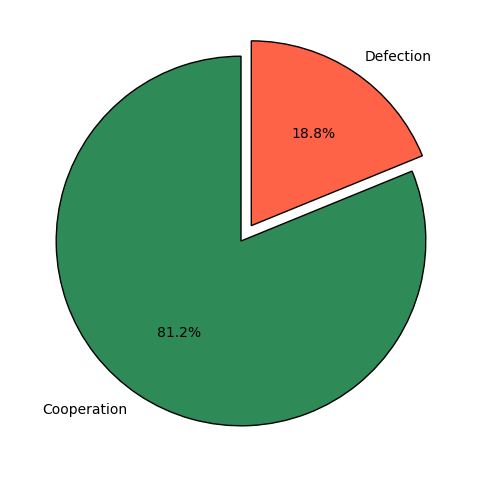
\includegraphics[width=7cm]{../poster/logos/qPie.png}
    \caption{Verteilung von Kooperation und Defektion des Q-Learning-Agenten}
    \label{fig:qverteilung}
\end{figure}

\subsection{Deep QLearning-Ergebnisse}
Der Deep Q-Learning-Agent geht als Sieger des Tuniers hervor mit durschnittlich $741597 / 2400 \approx 309$ Belohnungen pro Spiel. 
Die folgende Grafik zeigt die Verteilung von Kooperation und Defektion über alle Spiele im Turnier:
\begin{figure}[H]
    \centering
    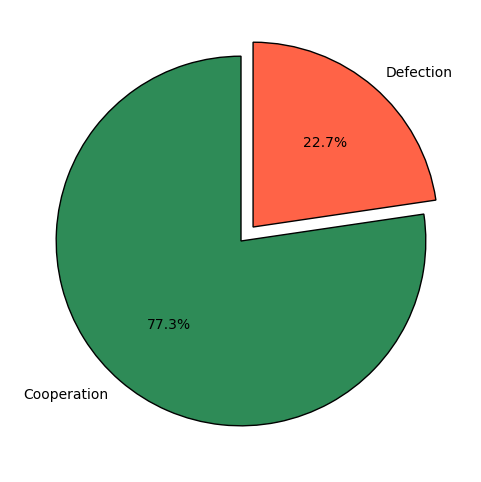
\includegraphics[width=7cm]{../poster/logos/deepqPie.png}
    \caption{Verteilung von Kooperation und Defektion des Deep Q-Learning-Agenten}
    \label{fig:deepqverteilung}
\end{figure}
Damit defektiert der Deep Q-Learning-Agent öfter als der Q-Learning-Agent, aber auch hier zeigt sich wieder: Es lohnt sich 
häufig zu kooperieren. 

Um besser zu verstehen wie der Deep Q-Learning-Agent agiert, kann man sich anschauen, wie er seine Strategie
je nach Gegner anpasst. Gegen die meisten Strategien setzt er auf langfristige Kooperation und defektiert nur sehr selten, es gibt
aber auch einige Ausnahmen:
Gegen den \textit{SoftMajorityAgent} wäre die beste Strategie abwechselnd zu koopieren und zu defektieren. Der
Deep Q-Learning-Agent erkennt dies und defektiert in fast 50\% der Runden. Gegen den \textit{ProvocativeAgent} defektiert er
fast immer, genauso wie gegen den \textit{TitForTatOppositeAgent}, was in beiden fällen auch sinnvolle Strategien sind. Gegen den 
\textit{TitForTwoTatsAgent} defektiert er ebenfalls in ungefähr 50\% der Runden. Teilweise ''verwechselt'' der Deep Q-Learning-Agent
seine Gegner und defektiert z.B. nur alle 2 Runden gegen den \textit{AlwaysCooperateAgent}. Gegen den \textit{AlwaysDefectAgent}
und den \textit{SpitefulAgent} hat er jedoch Probleme und kooperiert häufig. 

Insgesamt muss man anerkennen, dass ein ''perfektes'' Ergebnis nicht möglich ist. Im Verhalten des Deep Q-Learning-Agent erkennt man ebenfalls,
dass er zuerst ''testet'', gegen welchen Gegner er spielt. Das ist notwenig, um die Strategie anzupassen, führt aber auch zum Verlust von Punkten.
Beim \textit{SpitefulAgent} z.B. ist es aber schon zu spät, wenn man erkennt, dass dieser der Gegner ist. \\ \\
Durch diese Mischung aus langfristiger Kooperation und Ausnutzen von Schwachstellen in der gegnerischen Strategie ist der 
Deep Q-Learning-Agent in der Lage langfristig zu gewinnen und jede andere Strategie zu übertreffen.